\chapter{Anwendungen des Photons}

\setcounter{section}{6}
\setcounter{subsection}{0}
\setcounter{subsubsection}{1}
\setcounter{secnumdepth}{3}
% Boxen-Stile definieren
\tcbset{physikbox/.style={colback=blue!5!white, colframe=blue!75!black, fonttitle=\bfseries}}
\tcbset{mathebox/.style={colback=green!5!white, colframe=green!50!black, fonttitle=\bfseries}}
\tcbset{didaktikbox/.style={colback=yellow!5!white, colframe=yellow!50!black, fonttitle=\bfseries}}
\tcbset{hypobox/.style={colback=orange!5!white, colframe=orange!75!black, fonttitle=\bfseries}}
\tcbset{hinweisbox/.style={colback=gray!10!white, colframe=black!40!black, fonttitle=\bfseries}}

\subsection{Einleitung}

Photonen\index{Photon} sind nicht nur fundamentale Träger quantenphysikalischer Eigenschaften\index{Quantenphysikalische Eigenschaft} – sie bilden auch die Grundlage zahlreicher Anwendungen\index{Anwendung} in Technik\index{Technik}, Forschung\index{Forschung} und Alltag. In diesem Kapitel werden ausgewählte Einsatzfelder vorgestellt, in denen die Kontrolle\index{Photonenkontrolle}, Detektion\index{Photonendetektion} und Nutzung\index{Photonennutzung} einzelner Photonen eine zentrale Rolle spielt. Die Spannweite reicht von Lasertechnologie\index{Lasertechnologie} und Quantensensorik\index{Quantensensorik} über medizinische Bildgebung\index{Medizinische Bildgebung} bis hin zur optischen Kommunikation\index{Optische Kommunikation} und astronomischen Beobachtung\index{Astronomische Beobachtung}. Ziel ist es, die physikalischen Prinzipien\index{Physikalisches Prinzip} hinter diesen Anwendungen verständlich zu machen und ihre Bedeutung für Wissenschaft\index{Wissenschaft} und Gesellschaft\index{Gesellschaft} aufzuzeigen.

\subsection{Photonen in der Lasertechnologie}
\subsubsection{Funktionsprinzip von Lasern}

Der Begriff „Laser“\index{Laser} steht für \textbf{Light Amplification by Stimulated Emission of Radiation}\index{Light Amplification by Stimulated Emission of Radiation}. Ein Laser erzeugt Licht\index{Licht} nicht durch Glühen\index{Glühen} oder chemische Reaktionen\index{Chemische Reaktion}, sondern durch die gezielte Verstärkung von Photonen in einem aktiven Medium\index{Aktives Medium} – auf Basis der \emph{stimulierten Emission}\index{Stimulierte Emission}.

Die drei zentralen Prozesse\index{Einstein-Prozesse}, die Einstein\index{Einstein, Albert} bereits 1916 theoretisch beschrieb, sind:

\begin{itemize}
	\item \textbf{Spontane Emission}\index{Spontane Emission}: Ein angeregtes Atom\index{Atom} fällt ohne äußeren Einfluss in einen niedrigeren Zustand zurück und sendet ein Photon aus.
	\item \textbf{Absorption}\index{Absorption}: Ein Photon trifft auf ein Atom im Grundzustand und hebt es in einen angeregten Zustand.
	\item \textbf{Stimulierte Emission}: Ein Photon trifft auf ein bereits angeregtes Atom – dieses sendet daraufhin ein zweites, phasengleiches Photon aus.
\end{itemize}

Für eine effektive Lichtverstärkung\index{Lichtverstärkung} muss die stimulierte Emission dominieren. Dies erfordert eine sogenannte \emph{Besetzungsinversion}\index{Besetzungsinversion} – also mehr Atome im angeregten als im Grundzustand, was unter normalen Bedingungen nicht gegeben ist.

\medskip
\begin{tcolorbox}[physikbox, title={Stimulierte Emission als Grundlage des Lasers}]
	\label{box:grundlagedeslaser}
	Trifft ein Photon mit der passenden Energie auf ein angeregtes Atom, kann es dieses zur Aussendung eines zweiten Photons zwingen. Beide Photonen sind:
	\begin{itemize}
		\item \textbf{phasengleich}\index{Phasengleichheit} (gleiche Wellenphase),
		\item \textbf{frequenzgleich}\index{Frequenzgleichheit} (gleiche Energie) und
		\item \textbf{in gleicher Richtung}\index{Lichtausbreitungsrichtung} unterwegs.
	\end{itemize}
	Diese Eigenschaft erlaubt die kontrollierte Verstärkung von Licht – das Funktionsprinzip des Lasers.
\end{tcolorbox}

\subsubsection{Aufbau und Typen}

Ein Laser besteht im Wesentlichen aus drei funktionalen Komponenten:

\begin{itemize}
	\item \textbf{Aktives Medium:} Ein Material\index{Laser-Material}, dessen Atome oder Moleküle\index{Molekül} durch Energiezufuhr (Pumping\index{Pumping}) in angeregte Zustände gebracht werden können. Hier findet die stimulierte Emission statt.
	\item \textbf{Pumpeinheit}\index{Pumpeinheit}: Sie liefert die notwendige Energie, um eine Besetzungsinversion zu erzeugen. Möglich sind optisches\index{Optisches Pumpen}, elektrisches\index{Elektrisches Pumpen} oder chemisches Pumpen\index{Chemisches Pumpen}.
	\item \textbf{Resonator}\index{Resonator}: Zwei Spiegel\index{Spiegel}, die das Licht zwischen sich hin und her reflektieren. Einer der Spiegel ist teilweise durchlässig\index{Teilreflektierender Spiegel}, sodass ein Teil des verstärkten Lichts als Laserstrahl\index{Laserstrahl} austreten kann.
\end{itemize}

\begin{tcolorbox}[didaktikbox, title={Typenvielfalt von Lasern – ein Überblick}]
	\label{box:Typenvielfalt von Lasern}
	Laser unterscheiden sich hauptsächlich durch das aktive Medium:
	\begin{itemize}
		\item \textbf{Festkörperlaser}\index{Festkörperlaser} (z.\,B. Nd:YAG\index{Nd:YAG}): Hohe Leistung, verwendet in Industrie\index{Industrie} und Medizin\index{Medizin}.
		\item \textbf{Gaslaser}\index{Gaslaser} (z.\,B. Helium-Neon\index{Helium-Neon-Laser}, CO\textsubscript{2}\index{CO2-Laser}): Stabil und präzise, z.\,B. für Vermessung\index{Vermessung}.
		\item \textbf{Halbleiterlaser}\index{Halbleiterlaser} (z.\,B. Laserdiode\index{Laserdiode}): Kompakt, effizient, z.\,B. in CD/DVD-Playern\index{CD-Player}\index{DVD-Player} oder Laserpointern\index{Laserpointer}.
		\item \textbf{Faserlaser}\index{Faserlaser}: Licht wird in einer optischen Faser\index{Optische Faser} verstärkt – hohe Strahlqualität\index{Strahlqualität} bei robuster Bauweise.
		\item \textbf{Farbstofflaser}\index{Farbstofflaser}: Besonders flexibel in der Wellenlänge\index{Wellenlänge} durch organische Moleküle\index{Organisches Molekül} als Medium.
	\end{itemize}
\end{tcolorbox}

%index
\subsubsection{Anwendungen in Technik und Forschung}

\begin{tcolorbox}[didaktikbox, title={Anwendungen von Lasern — Technik (Überblick)}]	
	\label{box:lasertechnik}
	\begin{itemize}
		\item \textbf{Materialbearbeitung\index{Materialbearbeitung} (Schneiden, Schweißen, Härten):} Hohe Leistungsdichte, präziser Fokus, schmale Wärmeeinflusszone, gut automatisierbar.
		\item \textbf{Additive Fertigung\index{Additive Fertigung} (SLS/SLM, PBF):} Punktgenaues Aufschmelzen für komplexe, hochfeste Bauteile mit geringerem Materialverbrauch.
		\item \textbf{Messtechnik\index{Messtechnik} \& Metrologie\index{Metrologie} (Interferometrie, Lasertracker):} Präzise Längen-/Winkelmessungen bis in den nm-Bereich durch Kohärenz und Stabilität.
		\item \textbf{LIDAR\index{LIDAR} \& Distanzmessung\index{Distanzmessung}:} Schnelle 3D-Erfassung und robuste Reichweitenmessung (Autonomes Fahren, Drohnen, Geodäsie).
		\item \textbf{Glasfaserkommunikation\index{Glasfaserkommunikation}:} Sehr hohe Datenraten über große Distanzen (DWDM, kohärente Übertragung).
		\item \textbf{Oberflächenstrukturierung\index{Oberflächenstrukturierung} \& Lithografie\index{Lithografie}:} Direkte Mikro-/Nanostrukturierung („Laser-Direct-Write“), Prototyping, Mikromechanik.
		\item \textbf{Prozessanalytik\index{Prozessanalytik} (Raman\index{Raman-Spektroskopie}, LIBS\index{LIBS}):} Kontaktlose, schnelle Materialsensorik in-line ohne Probenvorbereitung.
		\item \textbf{Holografie\index{Holografie}, Displays\index{Displays} \& Projektion\index{Projektion}:} Hoher Kontrast, großer Farbraum, echte Hologramme und AR-Optiken.
		\item \textbf{Barcode-Scanning\index{Barcode-Scanning} \& Sensorik\index{Sensorik}:} Schnelle, kontrastreiche Abtastung in Handel, Logistik und Automation.
		\item \textbf{Ausrichten\index{Ausrichten} \& Justage\index{Justage}:} Der Laserstrahl als präzise Referenzgerade im Bau- und Maschinenbau.
	\end{itemize}
\end{tcolorbox}

\begin{tcolorbox}[didaktikbox, title={Anwendungen von Lasern — Forschung (Überblick)}] 
	\label{box:laser-app-forschung}
	\begin{itemize}
		\item \textbf{Spektroskopie\index{Spektroskopie} (Absorption, Fluoreszenz, Raman, CARS):} Schmalbandig/abstimmbar mit hoher Selektivität für Struktur- und Molekülinformationen.
		\item \textbf{Optische Pinzetten\index{Optische Pinzette} \& Mikromanipulation\index{Mikromanipulation}:} Kontaktlose Partikel-/Zellkontrolle durch stark fokussierte Strahlen.
		\item \textbf{Atomphysik\index{Atomphysik} (Laserkühlung\index{Laserkühlung}, MOT\index{Magneto-Optische Falle}, BEC\index{Bose-Einstein-Kondensat}):} Resonante Kühlung bis nK und präzise Kontrolle neutraler Atome.
		\item \textbf{Präzisionsmetrologie\index{Präzisionsmetrologie} (optische Uhren\index{Optische Uhr}, Frequenzkämme\index{Frequenzkamm}):} Extrem stabile Frequenzen und neue Zeit-/Längenstandards.
		\item \textbf{Nichtlineare Optik\index{Nichtlineare Optik} \& Attosekundenphysik\index{Attosekundenphysik}:} Frequenzumwandlung, Hochharmonische und ultraschnelle Dynamik.
		\item \textbf{Quantenoptik\index{Quantenoptik} \& Quantenkommunikation\index{Quantenkommunikation} (QKD\index{Quanten-Schlüsselverteilung}):} Einzelphotonen, Verschränkung, sichere Schlüsselverteilung.
		\item \textbf{Laser-Plasma\index{Laser-Plasma}, Beschleuniger\index{Teilchenbeschleuniger}, Fusion\index{Kernfusion}:} Extreme Intensitäten für dichte Plasmen, kompakte Beschleuniger und Trägheitsfusion.
		\item \textbf{Atmosphäre\index{Atmosphäre} \& Astronomie\index{Astronomie} (Lidar, Laser-Guide-Stars\index{Laser-Guide-Star}):} Sondierung von Aerosolen/Winden; adaptive Optik an Großteleskopen.
		\item \textbf{Biomedizinische Bildgebung\index{Biomedizinische Bildgebung} (2-Photonen, STED\index{STED-Mikroskopie}):} Tiefe, schonende und superauflösende Mikroskopie.
		\item \textbf{Femtochemie\index{Femtochemie} \& Pump-Probe\index{Pump-Probe-Experiment}:} Reaktionsdynamik in Echtzeit sichtbar machen.
	\end{itemize}
\end{tcolorbox}

%index
\subsection{Photonendetektoren und Sensorik\index{Photonendetektoren}\index{Sensorik}}

Die Detektion einzelner Photonen\index{Photon} ist eine Schlüsseltechnologie moderner Physik und Technik. Ob in der Astrophysik\index{Astrophysik}, der Quantenoptik\index{Quantenoptik}, der medizinischen Bildgebung\index{Medizinische Bildgebung} oder in der industriellen Qualitätskontrolle\index{Qualitätskontrolle} – empfindliche und präzise Sensoren entscheiden über die Aussagekraft eines Experiments oder den Erfolg einer Anwendung. In diesem Abschnitt werden zentrale Typen von Photonendetektoren, deren Funktionsweise sowie typische Anwendungen vorgestellt.

\subsubsection{Photomultiplier und Halbleiterdetektoren\index{Photomultiplier}\index{Halbleiterdetektoren}}

\textbf{Photomultiplier-Röhren (PMT)\index{PMT}} nutzen den photoelektrischen Effekt\index{Photoelektrischer Effekt}: Ein einfallendes Photon schlägt ein Elektron aus einer Photokathode\index{Photokathode} heraus. Dieses Elektron wird in einer Kaskade aus Dynoden\index{Dynode} vervielfacht und als makroskopisch messbares elektrisches Signal detektiert. PMTs bieten:

\begin{itemize}
	\item hohe Verstärkung (bis $10^6$–$10^8$),
	\item extrem hohe Empfindlichkeit im UV\index{Ultraviolett} bis sichtbaren Bereich,
	\item schnelle Reaktionszeiten im Nanosekundenbereich.
\end{itemize}

Nachteile sind die Empfindlichkeit gegenüber Magnetfeldern\index{Magnetfeld}, die Notwendigkeit einer Hochspannung\index{Hochspannung} und die mechanische Empfindlichkeit der Glasröhren.

\medskip

\textbf{Halbleiterdetektoren\index{Halbleiterdetektoren}}, insbesondere Avalanche-Photodioden (APDs\index{APD}) und Single-Photon Avalanche Diodes (SPADs\index{SPAD}), arbeiten ebenfalls mit dem photoelektrischen Effekt, aber innerhalb eines Halbleitermaterials\index{Halbleitermaterial}. Vorteile:

\begin{itemize}
	\item kompakte Bauform, robust und leicht integrierbar,
	\item gute Quanteneffizienz\index{Quanteneffizienz} (oft über 50\%),
	\item Möglichkeit zur Arrayschaltung\index{Arrayschaltung} (Pixel-Detektoren, SiPMs\index{SiPM}).
\end{itemize}

Sie sind die Basis moderner photonischer Sensorarrays\index{Sensorarray} in der Forschung und Industrie.
\begin{figure}[H]
	\centering
	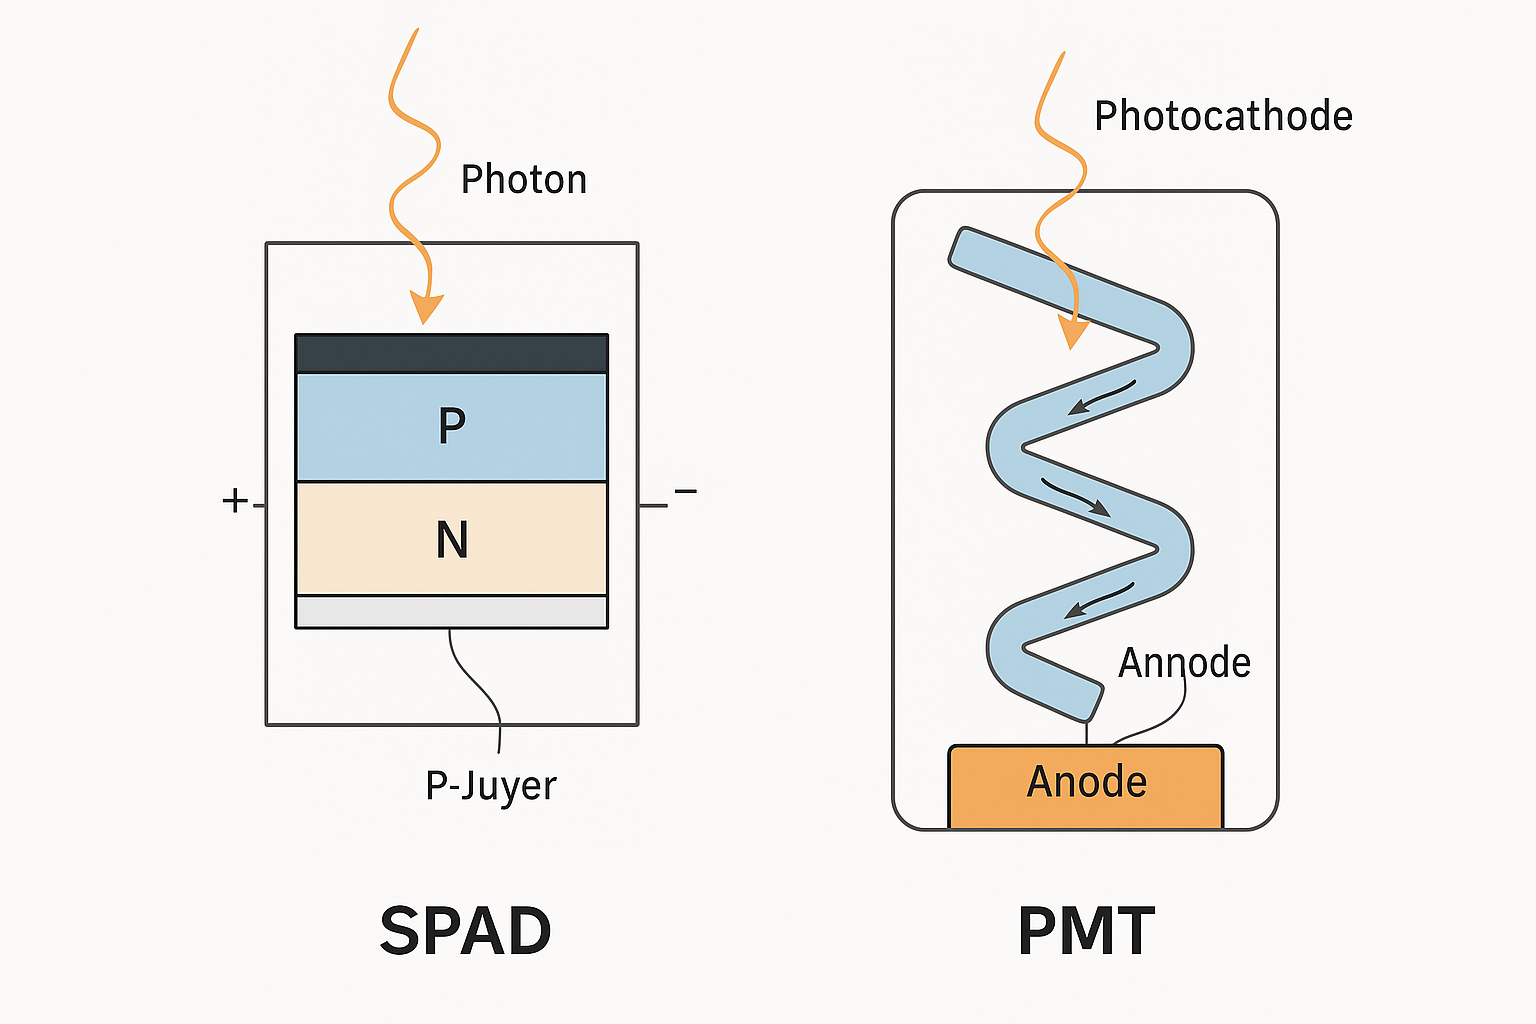
\includegraphics[width=0.9\linewidth]{bilder/SPAD-PMT.png}
	\caption{Schematischer Vergleich eines SPAD (Single-Photon Avalanche Diode, links) und eines PMT (Photomultiplier Tube, rechts). }
	\label{fig:spad_pmt}
\end{figure}
\begin{tcolorbox}[hinweisbox, title=Didaktischer Vergleich: SPAD vs. PMT]
	\label{box:vergleich SPAD}
	\small
	\begin{tabular}{p{0.48\linewidth} | p{0.48\linewidth}}
		\textbf{Single-Photon Avalanche Diode (SPAD)} & \textbf{Photomultiplier Tube (PMT)} \\
		\hline
		Halbleiterbauelement mit speziellem PN-Übergang\index{PN-Übergang}. & Vakuumröhre\index{Vakuumröhre} mit Photokathode und Verstärkungsstufen. \\
		\hline
		Ein Photon erzeugt ein Elektron-Loch-Paar\index{Elektron-Loch-Paar} im Sperrbereich\index{Sperrbereich}. & Ein Photon schlägt ein Elektron aus der Photokathode. \\
		\hline
		Das Elektron löst eine Avalanche-Lawine\index{Avalanche-Lawine} aus – ein elektrischer Impuls entsteht. & Das Elektron wird über mehrere Dynoden beschleunigt und vervielfacht. \\
		\hline
		Sehr hohe Zeitauflösung\index{Zeitauflösung}, ideal für kompakte, integrierte Quantensensoren\index{Quantensensor}. & Hohe Verstärkung, ideal für schwache Lichtquellen (z.\,B. Szintillatoren\index{Szintillator}). \\
		\hline
		Betrieb bei Raumtemperatur\index{Raumtemperatur}, einfache Integration in Chips\index{Chip}. & Benötigt Hochspannung, empfindlich gegen Magnetfelder. \\
		\hline
		Sehr gut geeignet für Arrays und bildgebende Systeme (SiPM). & Klassisch in der Kernphysik\index{Kernphysik}, Astronomie, PET\index{Positronen-Emissions-Tomographie} usw. verwendet. \\
	\end{tabular}
\end{tcolorbox}
\begin{tcolorbox}[didaktikbox, title=Begriffserklärung: Avalanche-Lawine]
	\label{box:avalanche}
	\small
	In einer \textbf{Avalanche-Lawine} (engl. avalanche breakdown) erzeugt ein freies Elektron im starken elektrischen Feld\index{Elektrisches Feld} eines Halbleiters durch Stoßionisation\index{Stoßionisation} weitere Elektronen. Dieser Prozess vervielfacht sich lawinenartig und führt zu einem messbaren Stromimpuls\index{Stromimpuls} – der Nachweis eines einzelnen Photons ist so möglich.
\end{tcolorbox}
\medskip
\begin{tcolorbox}[didaktikbox, title=Begriffserklärung: Szintillator]
	\label{box:szintillator}
	\small
	Ein \textbf{Szintillator} ist ein Material\index{Material}, das beim Auftreffen ionisierender Teilchen\index{Ionisierendes Teilchen} Licht\index{Licht} emittiert. Dieses sogenannte \emph{Szintillationslicht}\index{Szintillationslicht} kann von Photonendetektoren wie PMTs oder SiPMs registriert werden und ermöglicht die indirekte Messung von Strahlung\index{Strahlung}.
\end{tcolorbox}

%index111
\subsubsection{Einzelphotonenzählung und Quanteneffizienz\index{Einzelphotonenzählung}\index{Quanteneffizienz}}

Die Fähigkeit, \textbf{einzelne Photonen zu detektieren}\index{Photon} ist ein Meilenstein in der Quantentechnologie\index{Quantentechnologie}. Dabei ist nicht nur das „Zählen“ entscheidend, sondern auch die \textbf{Quanteneffizienz}\index{Quanteneffizienz}, also der Anteil der einfallenden Photonen, die tatsächlich ein messbares Signal erzeugen.
\medskip
\begin{tcolorbox}[physikbox, title=Physikalische Begriffe]
	\label{box:begriffe}
	\small
	\begin{itemize}
		\item \textbf{Einzelphotonenzählung (Single Photon Counting)}: Detektionsmethoden, bei denen jedes registrierte Signal einem einzelnen Photon zugeordnet werden kann.
		\item \textbf{Quanteneffizienz (QE)}: Verhältnis registrierter zu einfallenden Photonen, typischerweise wellenlängenabhängig\index{Wellenlänge}.
	\end{itemize}
\end{tcolorbox}

Technisch kommen dabei meist SPADs\index{SPAD} oder supraleitende Nanodetektoren\index{Supraleitender Nanodetektor} zum Einsatz. Letztere erreichen Quanteneffizienzen nahe 100\%, sind aber kryogen\index{Kryotechnik} zu betreiben.

\subsubsection*{Wie funktioniert Einzelphotonenzählung?}
\phantomsection
Bei der Einzelphotonenzählung wird jeder einzelne Photonenimpuls als diskretes Ereignis registriert. Der Detektor (z.\,B. ein SPAD) erzeugt bei Eintreffen eines Photons einen elektrischen Impuls – typischerweise eine kurze Spannungs- oder Stromspitze. Diese Impulse werden elektronisch ausgewertet:

\begin{itemize}
	\item Jeder Impuls entspricht einem detektierten Photon.
	\item Ein Zähler\index{Zähler} summiert diese Impulse über definierte Zeitintervalle.
	\item Das Ergebnis ist eine Photonenzahl pro Zeitintervall – z.\,B. „125 Photonen in 1 ms“.
\end{itemize}

Damit dies zuverlässig funktioniert, müssen die Impulse:
\begin{itemize}
	\item eine klare \textbf{Unterschreitungsschwelle} (Schwellwertdetektion\index{Schwellwertdetektion}) überschreiten,
	\item in der Zeit klar voneinander unterscheidbar sein (Totzeit\index{Totzeit} beachten),
	\item und dürfen nicht durch \textbf{thermisches Rauschen}\index{Thermisches Rauschen} oder Dunkelstrom\index{Dunkelstrom} verwechselt werden.
\end{itemize}
\medskip
\begin{tcolorbox}[didaktikbox, title=Was zählt als Photon? ]
	\label{box:photonenzaehlung}
	\small
	Nicht jeder registrierte Impuls stammt von einem Photon. Detektoren erzeugen auch \emph{Dunkelraten}\index{Dunkelrate} (Fehlsignale ohne Lichteinfall). Hochwertige Einzelphotonendetektoren erreichen jedoch Dunkelraten unter 100 Impulsen pro Sekunde und Quanteneffizienzen über 50–90\,\%.
\end{tcolorbox}

\subsubsection{Anwendungen in Industrie und Grundlagenphysik\index{Anwendungen!Photonendetektion}}

Die Anwendung photonischer Sensorik ist vielfältig:

\begin{itemize}
	\item \textbf{Grundlagenphysik\index{Grundlagenphysik}:} Detektion einzelner Photonen in Quantenoptik\index{Quantenoptik}-Experimenten (z.\,B. Antibunching\index{Antibunching}, HOM-Effekt\index{Hong-Ou-Mandel-Effekt}), Teilchendetektion in der Hochenergiephysik\index{Hochenergiephysik}, astronomische Beobachtungen\index{Astronomie} (z.\,B. Hubble\index{Hubble-Teleskop}, JWST\index{James-Webb-Weltraumteleskop}).
	\item \textbf{Industrielle Anwendungen\index{Industrie}:} Qualitätskontrolle\index{Qualitätskontrolle}, Laserscanner\index{Laserscanner}, Lichtvorhänge\index{Lichtvorhang}, Positionssensoren\index{Positionssensor}, Photonenspektroskopie\index{Photonenspektroskopie}.
	\item \textbf{Medizin und Biowissenschaften\index{Medizin}:} Fluoreszenzmikroskopie\index{Fluoreszenzmikroskopie}, PET-Scanner\index{Positronen-Emissions-Tomographie}, optische Tomographie\index{Optische Tomographie}.
\end{itemize}

\begin{tcolorbox}[hinweisbox, title=Hinweis zur Bedeutung der Detektionstechnologie]
	\label{box:detektionstechnologie}
	Die kontinuierliche Verbesserung der Photonen-Detektion ist eine Voraussetzung für den Fortschritt in der Quantenkommunikation\index{Quantenkommunikation}, der medizinischen Bildgebung\index{Medizinische Bildgebung} und der Grundlagenforschung\index{Grundlagenforschung}. Viele Entwicklungen der Quantentechnologie hängen direkt von der Fähigkeit ab, Photonen präzise und verlustarm nachzuweisen.
\end{tcolorbox}

\subsection{Photonen in der medizinischen Bildgebung\index{Photonen in der medizinischen Bildgebung}}

Photonen spielen eine zentrale Rolle in vielen bildgebenden Verfahren der modernen Medizin. Dabei reicht ihr Einsatzspektrum von hochenergetischer Röntgenstrahlung\index{Röntgenstrahlung} bis hin zu sanftem, sichtbarem Laserlicht\index{Laserlicht} in der optischen Diagnostik\index{Optische Diagnostik}. Unterschiedliche physikalische Prozesse – Absorption\index{Absorption}, Streuung\index{Streuung}, Fluoreszenz\index{Fluoreszenz} oder Emission\index{Emission} – werden genutzt, um Kontrast im Gewebe sichtbar zu machen oder pathologische Strukturen zu identifizieren.

%index
\subsubsection{Röntgen, CT und PET}

\textbf{Röntgenstrahlung}\index{Röntgenstrahlung} basiert auf hochenergetischen Photonen, die durch Absorption und Abschwächung beim Durchtritt durch den Körper ein Bild erzeugen. Dichteres Gewebe (z.\,B. Knochen) absorbiert mehr Photonen und erscheint heller auf dem Detektor.

\textbf{Computertomographie (CT)}\index{Computertomographie (CT)} erweitert diese Technik, indem sie aus vielen Röntgenprojektionen ein 3D-Bild rekonstruiert. Hierfür werden rotierende Röntgenquellen und Detektorarrays verwendet.

\textbf{Positronen-Emissions-Tomographie (PET)}\index{Positronen-Emissions-Tomographie (PET)} nutzt einen anderen Mechanismus: Radiopharmaka\index{Radiopharmakon} emittieren Positronen\index{Positron}, die mit Elektronen\index{Elektron} annihilieren – dabei entstehen zwei Photonen mit einer Energie von \SI{511}{keV}, die in entgegengesetzten Richtungen ausgesendet und durch Ringdetektoren erfasst werden. Aus der Koinzidenz der Detektion wird der Ursprungsort rekonstruiert.
\medskip
\begin{tcolorbox}[physikbox, title=Photonen bei der PET]
	\label{box:PET}
	\small
	Bei der PET entstehen zwei Gamma-Photonen mit \SI{511}{keV} bei der Annihilation von Elektron und Positron. Diese Photonen verlassen den Körper fast ungehindert und ermöglichen eine präzise Lokalisation des Stoffwechsels – z.\,B. bei Tumoren.
\end{tcolorbox}
\begin{figure}[H]
	\centering
	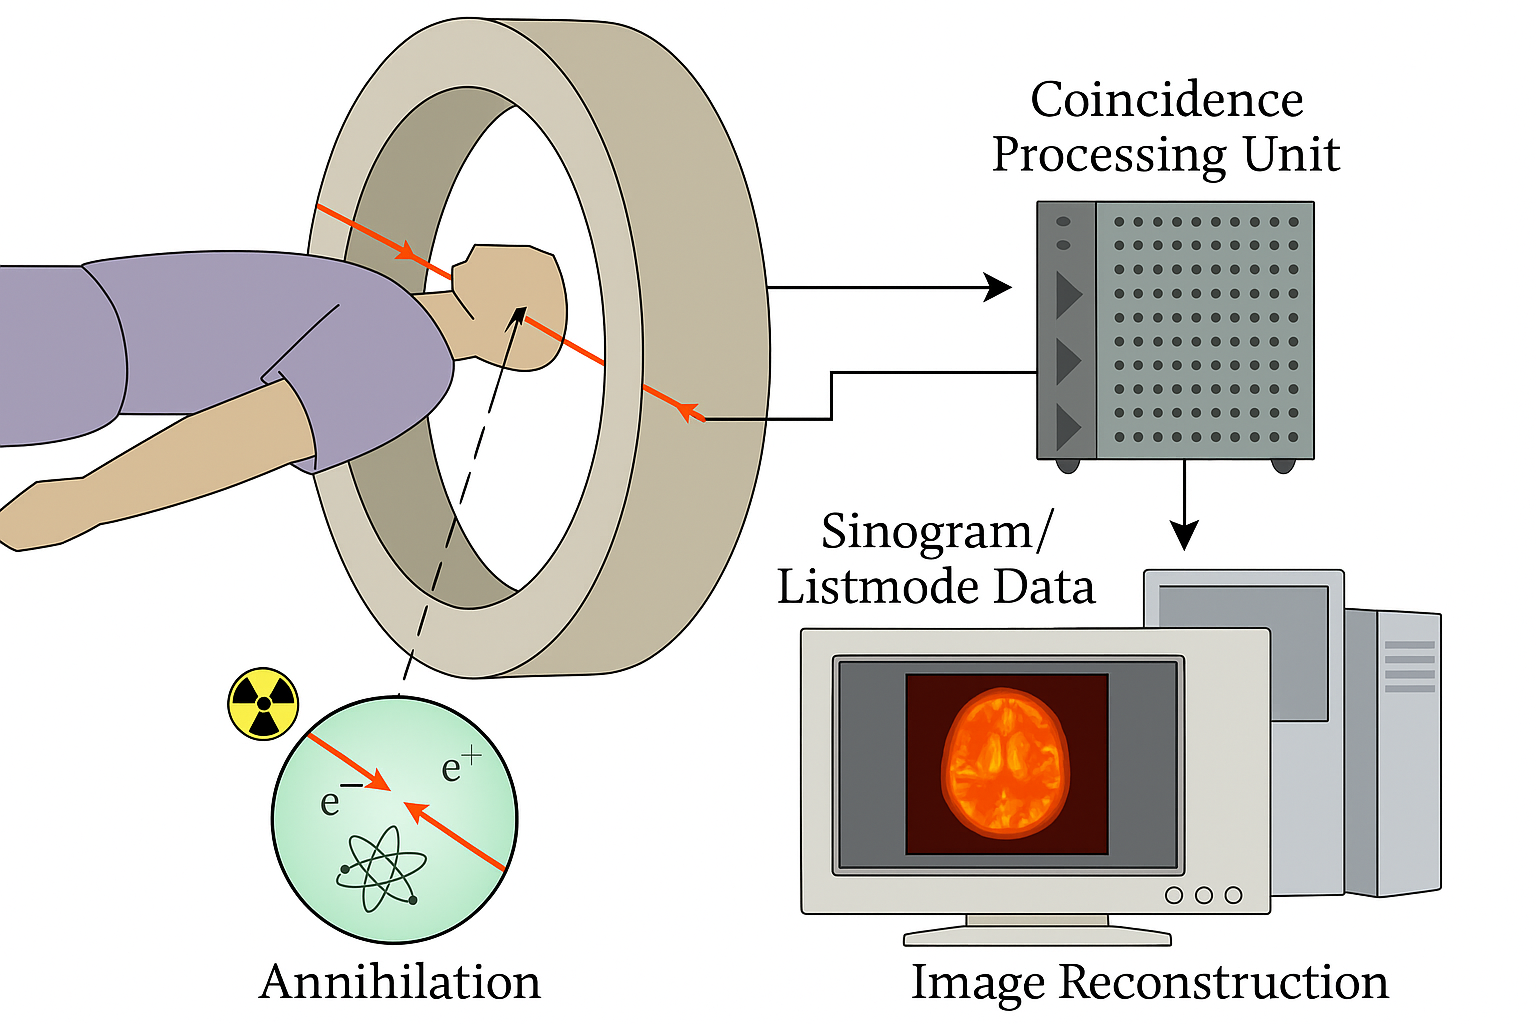
\includegraphics[width=0.85\linewidth]{bilder/petscan.png}
	\caption{Prinzip der Positronen-Emissions-Tomographie (PET): Ein verabreichtes Radiopharmakon emittiert ein Positron, das mit einem Elektron annihiliert. Dabei entstehen zwei Gamma-Photonen mit je \SI{511}{keV}, die in entgegengesetzten Richtungen ausgesendet und von Detektoren im PET-Ring registriert werden. Aus der Koinzidenz der Signale wird der Ursprungsort rekonstruiert.}
	\label{fig:pet_prinzip}
\end{figure}
\begin{tcolorbox}[didaktikbox, title=Begriffserklärung: Annihilation]
	\label{box:annihilation}
	\small
	Bei der \textbf{Annihilation} treffen ein Teilchen und sein Antiteilchen aufeinander und vernichten sich. Ihre Masse wird vollständig in Energie umgewandelt – meist in Form von Photonen. In der PET entsteht bei der Annihilation eines Elektrons mit einem Positron ein Photon-Paar mit je \SI{511}{keV}.
\end{tcolorbox}
\medskip
\begin{tcolorbox}[didaktikbox, title=Begriffserklärung: Radiopharmakon]
	\label{box:radiopharmakon}
	\small
	Ein \textbf{Radiopharmakon} ist ein radioaktiv markierter Wirkstoff, der gezielt in den Körper eingebracht wird. In der PET wird z.\,B. [\textsuperscript{18}F]FDG verwendet – eine Zucker-ähnliche Substanz, die sich in stoffwechselaktiven Geweben (wie Tumoren) anreichert. Die dort entstehenden Positronen liefern durch Annihilation das Bildsignal.
\end{tcolorbox}

\subsubsection{Optische Tomographie und Fluoreszenzbildgebung}

Im Gegensatz zur ionisierenden Strahlung setzen diese Verfahren auf sichtbares oder nahinfrarotes Licht.

\textbf{Diffuse optische Tomographie (DOT)}\index{Diffuse optische Tomographie (DOT)} verwendet Lichtquellen und Detektoren auf der Hautoberfläche. Die Photonen durchdringen das Gewebe, werden gestreut und absorbiert. Aus der Lichtverteilung kann auf die optischen Eigenschaften im Inneren geschlossen werden.

\textbf{Fluoreszenzbildgebung}\index{Fluoreszenzbildgebung} nutzt Substanzen (Fluorophore\index{Fluorophor}), die durch Licht angeregt werden und in einer anderen Wellenlänge wieder emittieren. Diese Methode erlaubt z.\,B. die Darstellung molekularer Prozesse oder Tumormarker.
\medskip
\begin{tcolorbox}[didaktikbox, title=Vorteil optischer Verfahren]
	\label{box:optisches Verfahren}
	\small
	Optische Methoden sind nicht-invasiv, strahlungsfrei und eignen sich besonders für Oberflächen- und funktionelle Bildgebung – z.\,B. bei Säuglingen, in der Neurodiagnostik oder der molekularen Bildgebung.
\end{tcolorbox}

\subsubsection{Laser in der Chirurgie und Diagnostik}

Laser\index{Laser} werden sowohl zur \textbf{Bildgebung} als auch zur \textbf{Gewebeeinwirkung} eingesetzt:

\begin{itemize}
	\item \textbf{Diagnostisch:} Konfokale Laser-Scanning-Mikroskopie\index{Konfokale Laser-Scanning-Mikroskopie}, optische Kohärenztomographie (OCT)\index{Optische Kohärenztomographie (OCT)}, Spektroskopie\index{Spektroskopie}.
	\item \textbf{Chirurgisch:} Gewebeschnitt, Koagulation, Ablation – je nach Wellenlänge, Pulsdauer und Leistung.
\end{itemize}

Laserchirurgie\index{Laserchirurgie} nutzt die präzise Fokussierung von Photonen zur gezielten Gewebeeinwirkung ohne mechanische Belastung. Typische Anwendungen sind:

\begin{itemize}
	\item Augenheilkunde\index{Augenheilkunde} (z.\,B. LASIK\index{LASIK}),
	\item Dermatologie\index{Dermatologie} (z.\,B. Tattoo-Entfernung\index{Tattoo-Entfernung}),
	\item Tumorchirurgie\index{Tumorchirurgie} (präzise Schnitte mit minimalem Blutverlust).
\end{itemize}

\begin{tcolorbox}[hinweisbox, title=Laserparameter]
	\label{box:laserparameter}
	\small
	Die Wirkung eines Lasers hängt stark von seiner Wellenlänge, Pulsdauer, Energie und Fokussierung ab. Kurze Pulse mit hoher Leistung ermöglichen präzise Schnitte, ohne umliegendes Gewebe zu beschädigen.
\end{tcolorbox}

\begin{figure}[H]
	\centering
	\includegraphics[width=0.85\linewidth]{bilder/oct.png}
	\caption{Schematische Darstellung der optischen Kohärenztomographie (OCT): Licht einer breitbandigen Quelle wird durch einen Strahlteiler aufgeteilt. Ein Teil trifft auf einen beweglichen Referenzspiegel (Referenzarm), der andere auf das zu untersuchende Gewebe (Sample). Die reflektierten Lichtanteile interferieren, und aus den Interferenzmustern wird das Tiefenprofil rekonstruiert. Das Ergebnis ist ein hochauflösendes Bild, z.\,B. der Netzhaut.}
	\label{fig:oct_prinzip}
\end{figure}

\begin{tcolorbox}[didaktikbox, title=Didaktische Erläuterung: Interferenz in der OCT]
	\label{box:interferenz_oct}
	\small
	\textbf{Interferenz} entsteht, wenn zwei Lichtwellen überlagert werden – je nach Phasenlage verstärken oder löschen sie sich aus. In der OCT wird diese Eigenschaft genutzt, um die Position reflektierender Strukturen im Gewebe mit hoher Präzision zu bestimmen.
	
	Nur wenn die optischen Weglängen im \emph{Sample Arm} und im \emph{Reference Arm} nahezu gleich sind, kommt es zu einem Interferenzsignal. Aus der gemessenen Intensität als Funktion der Referenzarm-Position ergibt sich ein sogenannter \textbf{A-Scan} – ein Tiefenprofil entlang einer Linie im Gewebe.
	
	Durch seitliches Verschieben des Messstrahls entsteht eine Vielzahl an A-Scans nebeneinander, die zu einem \textbf{B-Scan} (2D-Querschnitt) zusammengesetzt werden. So entsteht ein detailliertes Bild des untersuchten Gewebes – z.\,B. der Netzhaut.
\end{tcolorbox}

%index
\subsection{Photonen in der Kommunikation}
\index{Photonen in der Kommunikation}
\index{Datenübertragung}
\index{Quantenkommunikation}

Photonen bilden das Rückgrat moderner Datenübertragung – sowohl in klassischen Glasfasernetzen als auch in zukünftigen quantenbasierten Systemen. Die verlustarme Ausbreitung von Licht in optischen Medien, kombiniert mit hohen Bandbreiten und geringen Latenzen, macht die photonische Kommunikationstechnologie zu einem entscheidenden Faktor in der globalen Informationsinfrastruktur.

\subsubsection{Glasfaser und optische Netzwerke}
\index{Glasfaser}
\index{Optische Netzwerke}
\index{Totalreflexion}
\index{Wellenlängenmultiplexing}
\index{DWDM}
\index{EDFA}

\textbf{Glasfasern} leiten Licht durch Totalreflexion in einem dünnen Quarzfaserkern. Dabei können Photonen über Strecken von mehreren hundert Kilometern mit minimaler Dämpfung übertragen werden.

Vorteile:
\begin{itemize}
	\item extrem hohe Datenraten (Terabit/s),
	\item keine elektromagnetische Störung,
	\item geringe Dämpfung (z.\,B. \SI{0.2}{dB/km} bei \SI{1550}{nm}).
\end{itemize}

\textbf{Optische Netzwerke} nutzen Wellenlängenmultiplexing (DWDM), Verstärker (EDFA) und modulierte Lasersysteme, um große Datenmengen parallel und effizient zu übertragen – von Backbone-Netzen bis hin zu Glasfaseranschlüssen im Haus.
\medskip
\begin{tcolorbox}[physikbox, title=Totalreflexion in Glasfasern]
	\label{box:glasfaser}
	\small
	Die Lichtführung in einer Glasfaser erfolgt durch Totalreflexion an der Grenzfläche zwischen dem höherbrechenden Kern und dem Mantelmaterial. Der kritische Winkel bestimmt, ob das Licht innerhalb des Kerns „gefangen“ bleibt.
\end{tcolorbox}
\begin{figure}[H]
	\centering
	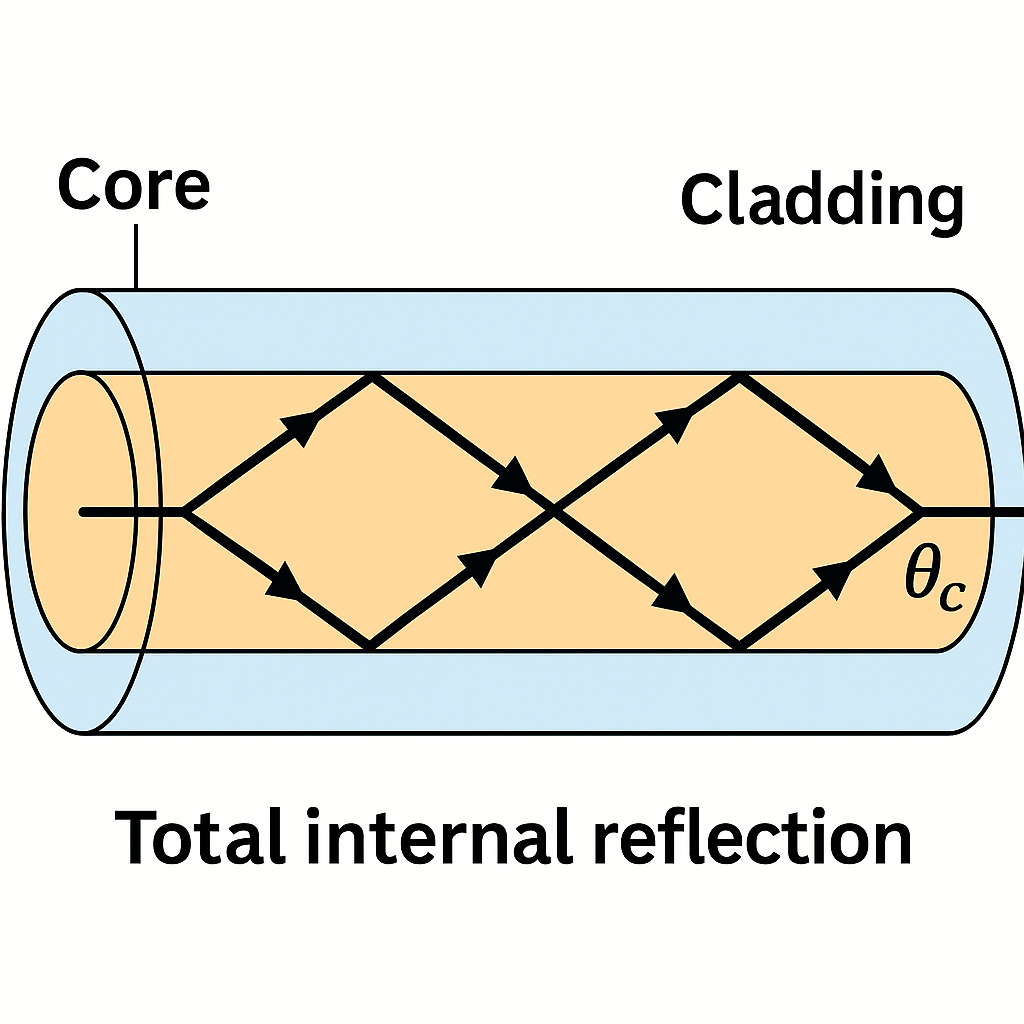
\includegraphics[width=0.8\linewidth]{bilder/glasfaser.png}
	\caption{Schematische Darstellung der Totalreflexion in einer Glasfaser: Das Licht (Photonen) wird im höherbrechenden Kern geführt und an der Grenzfläche zum Mantel (Cladding) vollständig reflektiert. So bleibt das Licht auch über große Strecken im Kern „gefangen“.}
	\label{fig:totalreflexion}
\end{figure}

%index
\subsubsection{Quantenkommunikation und QKD}\index{Quantenkommunikation}\index{QKD}\index{Photonen!Quantenkommunikation}\index{Polarisation!Photonen}\index{Verschränkung!Photonen}

Die \textbf{Quantenkommunikation} nutzt quantenmechanische Zustände von Photonen – etwa Polarisation oder Verschränkung –, um Informationen absolut abhörsicher zu übertragen.

\textbf{QKD (Quantum Key Distribution)} ist eine praktische Anwendung: Zwei Parteien (Alice und Bob) tauschen einen geheimen Schlüssel aus. Jeder Abhörversuch (Eve) verändert unweigerlich den Quantenzustand der Photonen und wird dadurch erkennbar.

\begin{tcolorbox}[didaktikbox, title=Was macht QKD sicher?] \index{QKD!Sicherheit}
	\label{box:qkd}
	\small
	Die Sicherheit beruht auf zwei quantenphysikalischen Prinzipien:
	\begin{itemize}
		\item \textbf{Nicht-Klonbarkeit}: Unbekannte Quantenzustände können nicht exakt kopiert werden.
		\item \textbf{Messstörung}: Jede Messung beeinflusst den Zustand – ein Abhörversuch stört das System messbar.
	\end{itemize}
\end{tcolorbox}

\textbf{BB84} ist das erste und bekannteste QKD-Protokoll. Es nutzt zufällige Polarisationen und Basiswechsel zur Erzeugung eines Schlüssels, der anschließend über einen klassischen Kanal verifiziert wird.

\medskip
\begin{tcolorbox}[didaktikbox, title=Wie funktioniert QKD (z.\,B. BB84)?] \index{QKD!BB84}\index{Quantenkommunikation!BB84}
	\label{box:wie funktioniert QKD}
	\small
	Beim BB84-Protokoll sendet Alice einzelne Photonen, deren Polarisation zufällig gewählt ist – z.\,B. horizontal ($\rightarrow$), vertikal ($\uparrow$), diagonal ($\searrow$) oder antidiagonal ($\nwarrow$). Bob misst ebenfalls in zufälligen Basen.
	
	Nur wenn Sender- und Empfängerbasis übereinstimmen, ergibt sich ein valides Bit. Nach dem Austausch vergleichen Alice und Bob (öffentlich) die verwendeten Basen und behalten nur die passenden. Aus diesen Bits entsteht der Schlüssel.
	
	Wird ein Photon abgehört, ändert sich seine Polarisation – dadurch erkennen Alice und Bob Störungen im Schlüssel und können Abhörversuche entdecken.
\end{tcolorbox}

%index
\subsubsection{Photonische Chips und zukünftige Systeme}\index{Photonische Chips}\index{Siliziumphotonik}\index{Photonen!Photonische Chips}\index{Datenverarbeitung!photonisch}\index{Logiksysteme!photonische}

Mit dem Aufkommen von \textbf{photonischen Chips} werden Lichtsignale nicht mehr durch Glasfasern allein, sondern direkt durch integrierte optische Schaltkreise geleitet. Diese ermöglichen:

\begin{itemize}
	\item kompakte, energieeffiziente Datenverarbeitung,
	\item lichtbasierte Logik- und Modulationssysteme,
	\item neue Konzepte für neuronale Netze und KI-Beschleuniger.
\end{itemize}

Photonische Chips kombinieren Laser, Modulatoren, Wellenleiter und Detektoren auf einem einzigen Substrat – oft Siliziumphotonik.

\begin{tcolorbox}[hinweisbox, title=Zukunft der photonischen Kommunikation] \index{Photonenbasierte Kommunikation}
	\label{box:Zukunft Kommunikation}
	\small
	Photonenbasierte Kommunikation ist nicht nur schneller als klassische Elektronik – sie wird zur Voraussetzung für sichere Quantennetzwerke, lichtbasierte Prozessoren und globale, abhörsichere Kommunikation.
\end{tcolorbox}

\subsection{Photonen in der astronomischen Beobachtung}\index{Astronomie!Photonen}\index{Photonen!Astronomie}\index{Photonen!astronomische Beobachtung}

Die Beobachtung von Photonen aus dem All ist das Fundament der modernen Astronomie. Da Photonen – anders als etwa Gravitationswellen oder Neutrinos – vergleichsweise leicht messbar sind, liefern sie einen Großteil unserer Informationen über das Universum. Ob sichtbares Licht, Radiostrahlung oder hochenergetische Gammastrahlen – jedes Photon, das die Erde erreicht, enthält eine Botschaft aus Raum und Zeit.

\subsubsection{Detektion von Photonen aus dem All}\index{Detektion!Photonen}\index{Photonen!Detektion!astronomisch}

Teleskope und Detektoren auf der Erde und im Weltall messen Photonen verschiedenster Wellenlängenbereiche:

\begin{itemize}
	\item \textbf{Optischer Bereich:} CCDs (Charge-Coupled Devices), CMOS-Sensoren
	\item \textbf{Infrarot und Radio:} Bolometer, Radioteleskope
	\item \textbf{Röntgen und Gamma:} Weltraumteleskope mit Szintillatoren und Halbleiterdetektoren
\end{itemize}

Die Analyse dieser Photonen liefert Informationen über Temperatur, Bewegung (Dopplerverschiebung), Zusammensetzung und Entfernung kosmischer Objekte.

\medskip
\begin{tcolorbox}[physikbox, title=Warum kommen manche Photonen nicht auf der Erde an?] \index{Erdatmosphäre!Photonenabsorption}\index{Photonen!Erdatmosphäre}
	\label{box:photonen auf erde}
	\small
	Die Erdatmosphäre ist für viele Wellenlängenbereiche nicht durchlässig – insbesondere für UV-, Röntgen- und Gammastrahlen. Deshalb müssen entsprechende Teleskope außerhalb der Atmosphäre – z.\,B. im Erdorbit – positioniert werden.
\end{tcolorbox}

%index
\subsubsection{Adaptive Optik, Spektroskopie und Teleskope}
\index{Adaptive Optik}
\index{Spektroskopie}
\index{Teleskope}
\index{Interferometrie}

\textbf{Teleskope} sammeln Photonen\index{Photon} und fokussieren sie auf Detektoren. Moderne Großteleskope (z.\,B. das VLT\index{Very Large Telescope (VLT)} oder ELT\index{Extremely Large Telescope (ELT)}) nutzen adaptive Optik, um die Bildqualität zu verbessern:

- \textbf{Adaptive Optik} kompensiert atmosphärische Störungen in Echtzeit durch deformierbare Spiegel.
- \textbf{Spektroskopie} zerlegt das Licht in seine Wellenlängen und erlaubt die Analyse chemischer Zusammensetzung, Temperatur und Bewegung von Himmelskörpern.
- \textbf{Interferometrie} kombiniert mehrere Teleskope zu einem virtuellen Riesenteleskop mit extrem hoher Winkelauflösung.
\begin{figure}[H]
	\centering
	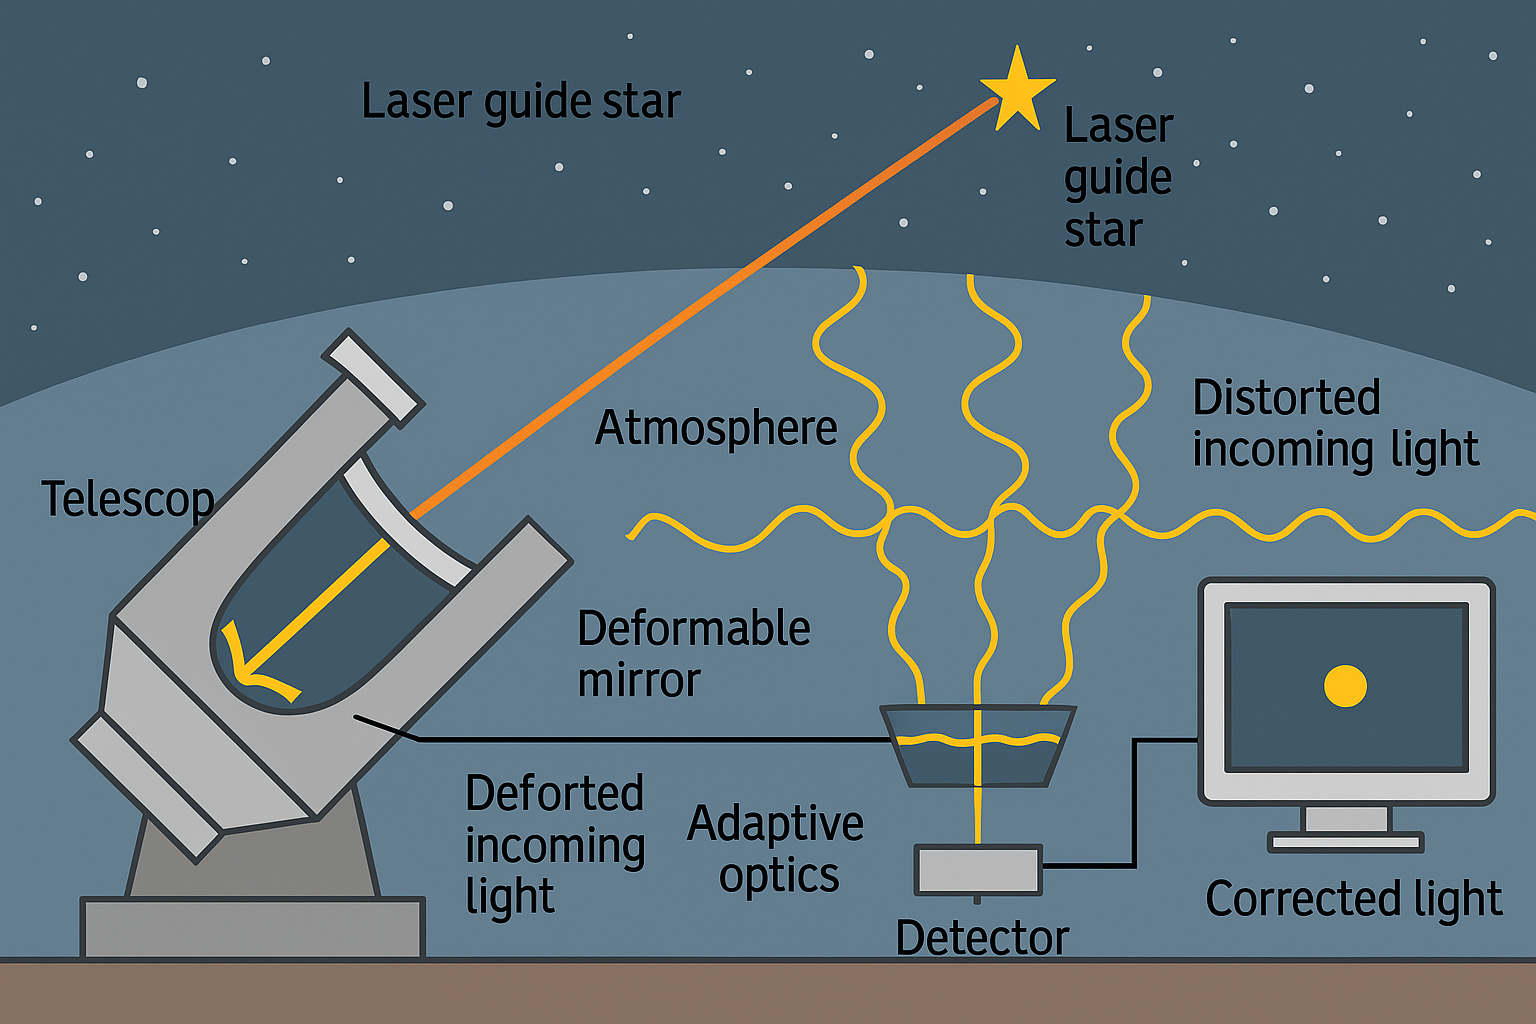
\includegraphics[width=0.9\linewidth]{bilder/Teleskop.png}
	\caption{Schematische Darstellung eines Teleskops mit adaptiver Optik. Ein Wellenfrontsensor analysiert Verzerrungen durch die Atmosphäre. Eine deformierbare Spiegeloberfläche korrigiert diese in Echtzeit, sodass ein scharfes Bild entsteht.}
	\label{fig:adaptive_optik}
\end{figure}

\begin{tcolorbox}[didaktikbox, title=Was zeigt ein Spektrum?]
	\label{box:was zeigt spektrum}
	\small
	Ein Spektrum\index{Spektrum} ist die Verteilung der Intensität der Photonen nach Wellenlängen. Typische Merkmale sind:
	\begin{itemize}
		\item \textbf{Emissionslinien}\index{Emissionslinien} $\rightarrow$ heiße, strahlende Gase,
		\item \textbf{Absorptionslinien}\index{Absorptionslinien} $\rightarrow$  kalte Gase vor heißen Quellen,
		\item \textbf{Rotverschiebung}\index{Rotverschiebung} $\rightarrow$  Bewegung des Objekts vom Beobachter weg.
	\end{itemize}
\end{tcolorbox}
\begin{figure}[H]
	\centering
	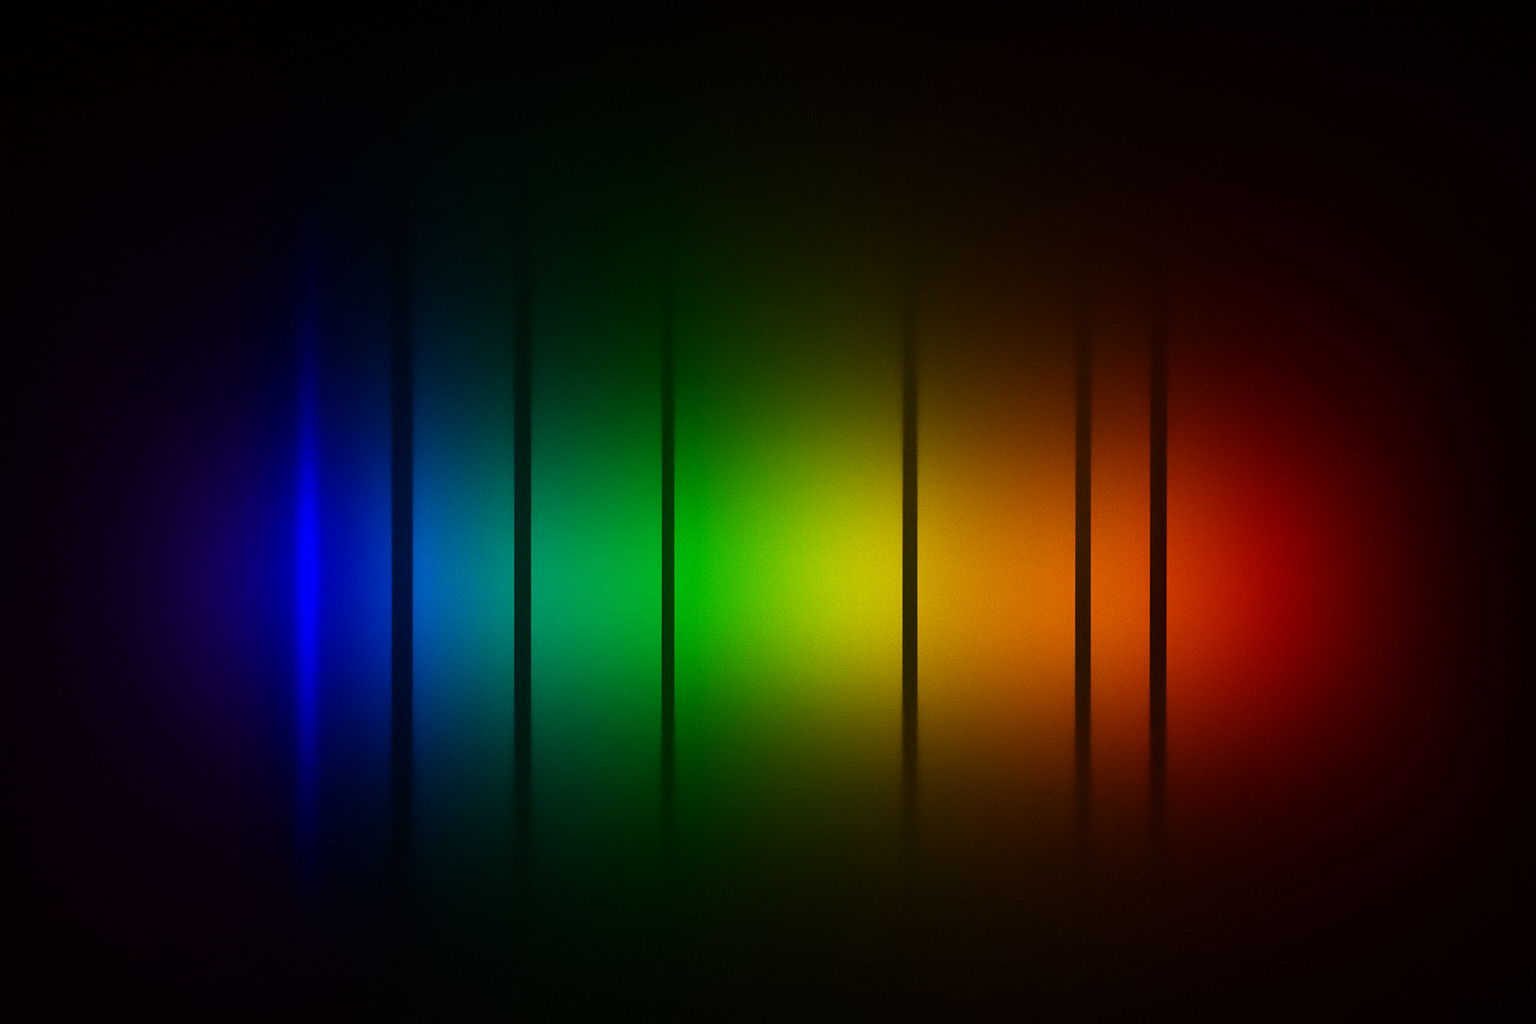
\includegraphics[width=0.9\linewidth]{bilder/emissionslinien.png}
	\caption{Emission von Strahlungslinien eines glühenden  Wasserstoffgases.}
	\label{fig:emission_hydrogen}
\end{figure}

\begin{tcolorbox}[physikbox, title=Spektrallinien und Rotverschiebung]
	\label{box:spektrallinien}
	\small
	\begin{itemize}
		\item \textbf{Emissionslinien} entstehen, wenn Atome spezifische Photonen aussenden. Diese Linien sind hell und charakteristisch für das jeweilige Element\index{Elementspektrum}.
		\item \textbf{Absorptionslinien} entstehen, wenn Photonen bestimmter Frequenzen von einem durchstrahlten Gas absorbiert werden – sie fehlen dann im Spektrum.
		\item \textbf{Rotverschiebung:} Entfernt sich eine Lichtquelle, verschieben sich alle Linien zu längeren Wellenlängen – in Richtung Rot. Dies wird zur Messung kosmischer Bewegungen\index{Kosmische Expansion} genutzt.
	\end{itemize}
\end{tcolorbox}

%index
\subsubsection{Photonen in der Gravitationswellenastronomie}
\index{Gravitationswellenastronomie}
\index{Gravitationswellen}
\index{Photon}
\index{Interferometer}
\index{LIGO}
\index{Virgo}

Gravitationswellen sind fundamentale Verzerrungen der Raumzeit\index{Raumzeit} – ausgelöst durch beschleunigte Massen, etwa bei der Verschmelzung Schwarzer Löcher\index{Schwarzes Loch}. Sie sind keine elektromagnetischen Wellen und bestehen nicht aus Photonen. Dennoch sind es gerade Photonen, die den Nachweis dieser Phänomene ermöglichen: als präzise Messsonden in hochsensitiven Interferometern.

\vspace{0.5em}
\textbf{LIGO, Virgo und andere Gravitationswellen-Detektoren} nutzen kilometerlange Laserinterferometer, um winzige Veränderungen der Raumzeit zu messen. Dabei werden Laserstrahlen (bestehend aus kohärenten Photonen) in zwei senkrecht zueinander verlaufende Arme gesendet, an Spiegeln reflektiert und am Ausgang überlagert. Eine vorbeiziehende Gravitationswelle verändert minimal die Armlängen – und damit das Interferenzmuster.

\medskip
\begin{tcolorbox}[physikbox, title=Photonen als Messwerkzeug für Raumkrümmung]
	\label{box:messwerkzeug}
	\small
	Laserinterferometer wie LIGO nutzen Photonen, um Differenzen in der Armlänge von bis zu \SI{1e-19}{m} zu detektieren – das ist etwa tausendmal kleiner als ein Proton\index{Proton}. Der Zeitunterschied, den ein Photon auf zwei Wegen durch das Interferometer benötigt, ändert sich messbar durch eine vorbeiziehende Gravitationswelle.
\end{tcolorbox}

Diese Technik beruht auf der Interferenz\index{Interferenz} kohärenter Lichtwellen. Sobald die beiden Teilstrahlen nach ihrem Lauf durch die beiden Arme wieder zusammengeführt werden, kommt es – je nach Phasenverschiebung – zu konstruktiver oder destruktiver Interferenz. Schon kleinste Änderungen der optischen Weglängen beeinflussen dieses Muster. Auf diese Weise lassen sich selbst winzige Krümmungen der Raumzeit nachweisen.

\vspace{0.5em}
Dank dieser photonengestützten Präzisionsmessung wurden erstmals Ereignisse wie die Verschmelzung Schwarzer Löcher, die Kollision von Neutronensternen\index{Neutronenstern} oder Spuren des kosmischen Gravitationshintergrunds\index{Kosmischer Gravitationshintergrund} experimentell nachgewiesen. Photonen machen also sichtbar, was ansonsten jenseits direkter Beobachtung läge – ein weiterer Beleg für ihre zentrale Rolle in der modernen Physik.

\medskip
\begin{tcolorbox}[didaktikbox, title=Wie funktioniert ein Interferometer? \label{box:interferometer}]
	\small
	Ein Interferometer nutzt das Prinzip der Überlagerung (Interferenz) von Lichtwellen, um kleinste Längenunterschiede sichtbar zu machen. 
	
	\begin{itemize}
		\item Ein Laserstrahl\index{Laser} wird mithilfe eines Strahlteilers in zwei Teilstrahlen aufgespalten.
		\item Diese laufen entlang zweier rechtwinklig zueinander stehender Arme zu Spiegeln, werden reflektiert und wieder zusammengeführt.
		\item Wenn sich die optischen Weglängen der beiden Arme genau entsprechen, löschen sich die Wellen teilweise oder vollständig aus – das Interferenzmuster ist konstant.
		\item Verändert sich eine Armlänge minimal (z.\,B. durch eine Gravitationswelle), verschiebt sich die Phase einer Welle, und das Interferenzmuster ändert sich messbar.
	\end{itemize}
	
	So können selbst winzige Längenänderungen – kleiner als ein Atomdurchmesser – durch die Analyse der Lichtintensität am Detektor erkannt werden. Das Licht dient dabei als präzise „Messlatte“ im Raum.
\end{tcolorbox}

\medskip
\begin{tcolorbox}[didaktikbox, title=Warum sind Photonen so genau messbar? \label{box:photonen_genau}]
	\small
	Photonen sind ideale Messwerkzeuge – aus mehreren Gründen:
	
	\begin{itemize}
		\item \textbf{Hohe Kohärenz:} Laserlicht besteht aus kohärenten Photonen – also Wellen mit exakt gleicher Frequenz und stabiler Phasenlage. Das ermöglicht extrem empfindliche Interferenzeffekte.
		\item \textbf{Geringe Wechselwirkung:} Photonen wechselwirken kaum mit Materie. Dadurch lassen sich lange Laufstrecken realisieren, ohne dass sie gestört oder abgelenkt werden.
		\item \textbf{Quantennatur:} Einzelne Photonen sind diskrete Quantenobjekte\index{Quantennatur}. Ihre Erfassung erzeugt eindeutige, zählbare Signale – ideal für präzise Zeit- oder Ortsmessungen.
		\item \textbf{Lichtgeschwindigkeit als Konstante:} Die Geschwindigkeit von Photonen im Vakuum ist konstant\index{Lichtgeschwindigkeit}. Dadurch eignen sie sich als natürliche „Zeit- und Längenmaßstäbe“.
	\end{itemize}
	
	Diese Eigenschaften machen Photonen unverzichtbar in der modernen Messtechnik – vom Interferometer über Quantensensoren\index{Quantensensor} bis hin zu optischen Atomuhren\index{Optische Atomuhr}.
\end{tcolorbox}

\subsubsection{Fazit}

Photonen sind nicht nur zentrale Objekte der modernen Physik, sondern auch unverzichtbare Werkzeuge in Wissenschaft, Technik, Medizin und Kommunikation. Dieses Kapitel hat gezeigt, wie vielfältig und präzise Photonen kontrolliert, erzeugt und detektiert werden können:

\begin{itemize}
	\item In der \textbf{Lasertechnologie}\index{Lasertechnologie} ermöglichen stimulierte Emission und kohärente Lichtverstärkung Anwendungen von der Materialbearbeitung bis zur Quantenoptik\index{Quantenoptik}.
	\item \textbf{Photonendetektoren}\index{Photonendetektor} wie SPADs\index{SPAD} oder PMTs\index{Photomultiplier (PMT)} erlauben die Einzelphotonenzählung mit hoher Quanteneffizienz\index{Quanteneffizienz} – Grundlage für Quantentechnologien\index{Quantentechnologie} und präzise Bildgebung.
	\item In der \textbf{medizinischen Diagnostik}\index{Medizinische Diagnostik} werden Photonen zur Bildgebung mit hoher räumlicher Auflösung und minimaler Belastung eingesetzt – vom Röntgen\index{Röntgen} bis zur Fluoreszenzmikroskopie\index{Fluoreszenzmikroskopie}.
	\item Die \textbf{optische Kommunikation}\index{Optische Kommunikation} nutzt Photonen zur schnellen, verlustarmen und abhörsicheren Datenübertragung – in Glasfasern\index{Glasfaser} wie auch in Quantenkommunikationssystemen\index{Quantenkommunikation}.
	\item In der \textbf{astronomischen Beobachtung}\index{Astronomie} liefern Photonen entscheidende Informationen über Struktur, Bewegung und Zusammensetzung des Universums – bis hin zum Nachweis von Gravitationswellen durch interferometrische Messung.
\end{itemize}

Die Fähigkeit, einzelne Photonen gezielt zu erzeugen, zu lenken und zu messen, markiert einen technologischen Wendepunkt: Von klassischen Anwendungen bis zur Quanteninformationstechnik\index{Quanteninformationstechnik} eröffnet das Photon neue Horizonte – in Forschung, Industrie und Gesellschaft.



